\chapter{Genomic prediction}

Let's review the basic approach we use in genome-wide association
mapping.

\begin{itemize}

\item We measure both the phenotype, $y_i$, of individual $i$ and its
  genotype at a large number of loci, where $x_{ij}$ is the
  individual's genotype at locus $j$.

\item We regress phenotype on genotype one locus at a time, using a
  random effect to correct for phenotypic similarities that reflect
  relatedness rather than similarity in genotype. 
\[
y_i^{(k)} = x_{ij}\beta_j + \phi^{(k)} + \epsilon_i \quad .
\]

\end{itemize}

Keep in mind this is a highly idealized schematic of how GWAS analyses
are actually done.\footnote{Remember, also, that in analyses of human
  disease, a case-control approach is often used rather than the
  regression approach I've been focusing on.} If you want to do GWAS
for real, you should take a look at
GEMMA~(\url{http://www.xzlab.org/software.html})\index{GEMMA} or
TASSEL~(https://www.maizegenetics.net/tassel).\index{TASSEL} One
important way in which what I've presented is a simplification is that
in a real GWAS analysis, you'd estimate the effects of every locus
simultaneously, which raises an interesting problem.

In a typical GWAS analysis\footnote{In humans at least}, you will have
measured the phenotype of a few thousand individuals, but you will
have genotyped those individuals at several hundred thousand
loci. Lango Allen et al.~\cite{LangoAllen-etal-2010} report results
from a large analysis of height variation in humans, 183,727
individuals genotyped at 2,834,208 loci. What's the problem here?

There are more predictors~(loci) than observations~(individual
phenotypes). If you remember some basic algebra, you'll remember that
you can't solve a set of linear equations unless you have the same
number of equations as unknowns. For example, you can't solve a set of
three equations that has five unknowns. There's a similar phenomenon
in statistics when we're fitting a linear regression. In statistics we
don't ``solve'' an equation. We find the best fit in a regression, and
we can do so in a reasonable way so long as the number of observations
exceeds the number of variables included in our regression. To put a
little mathematical notation to it, if $n$ is the number of
observations and $p$ is the number of regression parameters we hope to
estimate, life is good (meaning that we can estimate the regression
parameters) so long as $n > p$.\footnote{And the more that $n$ exceeds
  $p$ the better, the more accurate our estimates of the regression
  parameters will be.} The typical situation we encounter in GWAS is
that $n < p$, which means we have to be really sneaky. Essentially
what we do is that we find a way for the data to tell us that a lot of
the parameters don't matter and we fit a regression only to the ones
that do, {\it and\/} we set things up so that the remaining number of
parameters is less than $n$. If that all sounds a little hoky, trust
me it isn't. There are good ways to do it and good statistical
justification for doing it\footnote{And biological justification for
  doing it in GWAS.}, but the mathematics behind it gets pretty hairy,
which is why you want to use GEMMA or TASSEL for a real GWAS. We'll
ignore this part of the challenge associated with GWAS and focus on
another one: complex traits often are influenced by a very large
nubmer of loci.

\section*{Genetics of complex traits}

Let's return to that Lango Allen et al.~\cite{LangoAllen-etal-2010}
GWAS on height in humans. They identified at least 180 loci associated
with differences in height. Moreover, many of the variants are closely
associated with genes that are part of previously identified pathways,
e.g., Hedgehog signaling,\footnote{``The Hedgehog signaling pathway is
  a signaling pathway that transmits information to embryonic cells
  required for proper cell differentiation.''
  \url{https://en.wikipedia.org/wiki/Hedgehog_signaling_pathway}} or
that were previously identified as being involved in skeletal growth
defects. A more recent study by Wood et al.~\cite{Wood-etal-2014}
synthesized results from 79 studies involving 253,288 individuals and
identified 697 variants that were clustered into 423 loci affecting
differences in height.\footnote{It's worth noting that even this is
  likely to be an underestimate of the number of loci associated with
  height variation in humans because all of the individuals included
  in the analysis were of European ancestry.} Think about what that
means. If you know my genotype at only one of those 697 variants, you
know next to nothing about how tall I am. But what if you knew my
genotype for all of those variants? Then you should be able to do
better.\index{Genome-wide association study!human height}

The basic idea is fairly simple. When you do a full GWAS and estimate
the effects at every locus simultaneously, you are essentially
performing a multiple regression of phenotype on all of the loci
you've scored simultaenously instead of looking at them one at a
time. In equation-speak,
\[
y_i^{(k)} = \sum_j x_{ij}\beta_j + \phi^{(k)} + \epsilon_i \quad .
\]
Now think a bit more about what that equation means. The $\phi^{(k)}$
and $\epsilon_i$ terms represent random variation, in the first case
variation that is correlated among individuals depending on how
closely related they are and in the second case variation that is
purely random. The term $\sum_j x_{ij}\beta_j$ reflects systematic
effects associated with the genotype of individual $i$. In other
words, if we know individual $i$'s genotype, i.e., if we know $x_{ij}$
we can predict what phenotype it will have, namely
$\mu_i = \sum_j x_{ij}\beta_j$. Although we know there will be
uncertainty associated with this prediction, $\mu_i$ is our best guess
of the phenotype for that individual, i.e., our genomic prediction or
polygenic score. In the case of height in human beings, it turns out
that the loci identified in Wood et al.~\cite{Wood-etal-2014} account
for about 16 percent of variation in height.\footnote{In Europe the
  heritability of height at age 20 is about 80
  percent~\cite{Jelenkovic-etal-2016}.}\index{genomic predictioon}
\index{polygenic score}

\subsection*{A toy example}

To make all of this more concrete, we'll explore a toy example using
the highly simplified one locus at a time approach to GWAS with a
highly simplified example of the multiple regression approach to
GWAS. You'll find the {\tt R} code used to create and analyze this
simple example at
\url{http://darwin.eeb.uconn.edu/eeb348-resources/genomic-prediction.R}
If you {\tt source("genomic-prediction.R")} it will

\begin{itemize}

\item Generate a random dataset with 100 individuals and 20 loci, 5 of
  which influence the phenotype. The effect of one ``1'' allele at
  locus 1 is 1, at locus 2 -1, at locus 3 0.5, at locus 4 -0.5, and at
  locus 5 0.25. The standard deviation of the phenotype around the
  predicted mean is 0.1.

\item Run the locus-by-locus regression for each locus and store the
  results (mean and 95\% credible interval) in ``results.csv'' and
  retain the results in {\tt results}. {\tt results} is sorted in by
  the magnitude of the posterior mean, so that loci with the largest
  estimated effect occur at the top and loci with the smallest effect
  occur at the bottom.

\item Run the multiple regression and store the results in {\tt fit}. 
    
\end{itemize}

If you look at the code, you'll see that I use {\tt stan\_lm()} for the
locus by locus regression rather than the {\tt Stan} code you used in
Project \#6. That's because I simulate the data without family
structure, so there's no need to include the family random effect.

Table~\ref{table:single} shows results of the locus by locus analysis
from my run of {\tt genomic-prediction.R}. Your results will vary a
bit, both because the Monte Carlo analysis of the data won't be
precisely the same every time and because the data you generate in the
simulation will be a bit different from the data I generated for this
analysis.

% latex table generated in R 3.5.3 by xtable 1.8-3 package
% Sun Apr 28 11:27:43 2019
\begin{table}[ht]
\centering
\begin{tabular}{rrrr}
  \hline
 & mean & 2.5\% & 97.5\% \\ 
  \hline
locus\_1 & 1.01 & 0.76 & 1.27 \\ 
  locus\_2 & -0.97 & -1.12 & -0.82 \\ 
  locus\_3 & 0.63 & 0.34 & 0.91 \\ 
  locus\_4 & -0.42 & -0.71 & -0.13 \\ 
  locus\_5 & 0.42 & 0.11 & 0.72 \\ 
  locus\_14 & 0.23 & -0.07 & 0.52 \\ 
  locus\_8 & -0.17 & -0.47 & 0.13 \\ 
  locus\_6 & -0.14 & -0.47 & 0.18 \\ 
  locus\_20 & -0.13 & -0.46 & 0.18 \\ 
  locus\_19 & -0.12 & -0.44 & 0.20 \\ 
  locus\_10 & 0.11 & -0.22 & 0.44 \\ 
  locus\_18 & 0.09 & -0.22 & 0.40 \\ 
  locus\_9 & -0.09 & -0.39 & 0.22 \\ 
  locus\_12 & -0.09 & -0.41 & 0.26 \\ 
  locus\_15 & -0.07 & -0.37 & 0.23 \\ 
  locus\_11 & -0.07 & -0.40 & 0.27 \\ 
  locus\_7 & -0.04 & -0.34 & 0.27 \\ 
  locus\_16 & -0.04 & -0.35 & 0.28 \\ 
  locus\_13 & 0.03 & -0.29 & 0.36 \\ 
  locus\_17 & 0.01 & -0.32 & 0.35 \\ 
   \hline
\end{tabular}
\caption{Sample results for locus by locus analysis of genetic
  associations using {\tt genomic-prediction.R}}\label{table:single}
\end{table}

For this simulated data set the 5 loci with the largest estimated
effect are the 5 loci for which I specified an effect, but that isn't
always the case. You may well find that a locus that didn't have a
specified effect is one of the top 5. Furthermore, even though this
time the locus by locus approach picked out the right top 5 loci, {\tt
  locus\_14} has an effect that is quite large, the the credible
interval associated with it only overlaps 0, by a bit. It would be
tempting to think that it is worth investigating further. It wouldn't
be as tempting to look at any of the other loci, but a lot of them
have fairly large effects given that the entire observed range of
phenotypes in this data set is -2.8 to 3.2.

Since you've already run {\tt source("genomic-predicition.R")}, you
can now run {\tt plot\_posterior\_predict(fit\_list[[1]])} to plot
phenotype predictions at locus 1 versus the observed phenotype for
each individual~(Figure~\ref{fig:locus-1}). You can see that there is
a relationship between an individual's genotype at this locus, but you
can also see that it's pretty weak. Compare that to the relationship
between phenotype and genotype at {\tt locus\_17}, though, and you'll
see that the genotype at locus 17 doesn't give you any information
about phenotype while the genotype at locus 1 at least gives you a
little~(Figure~\ref{fig:locus-17}).

\begin{figure}
  \begin{center}
    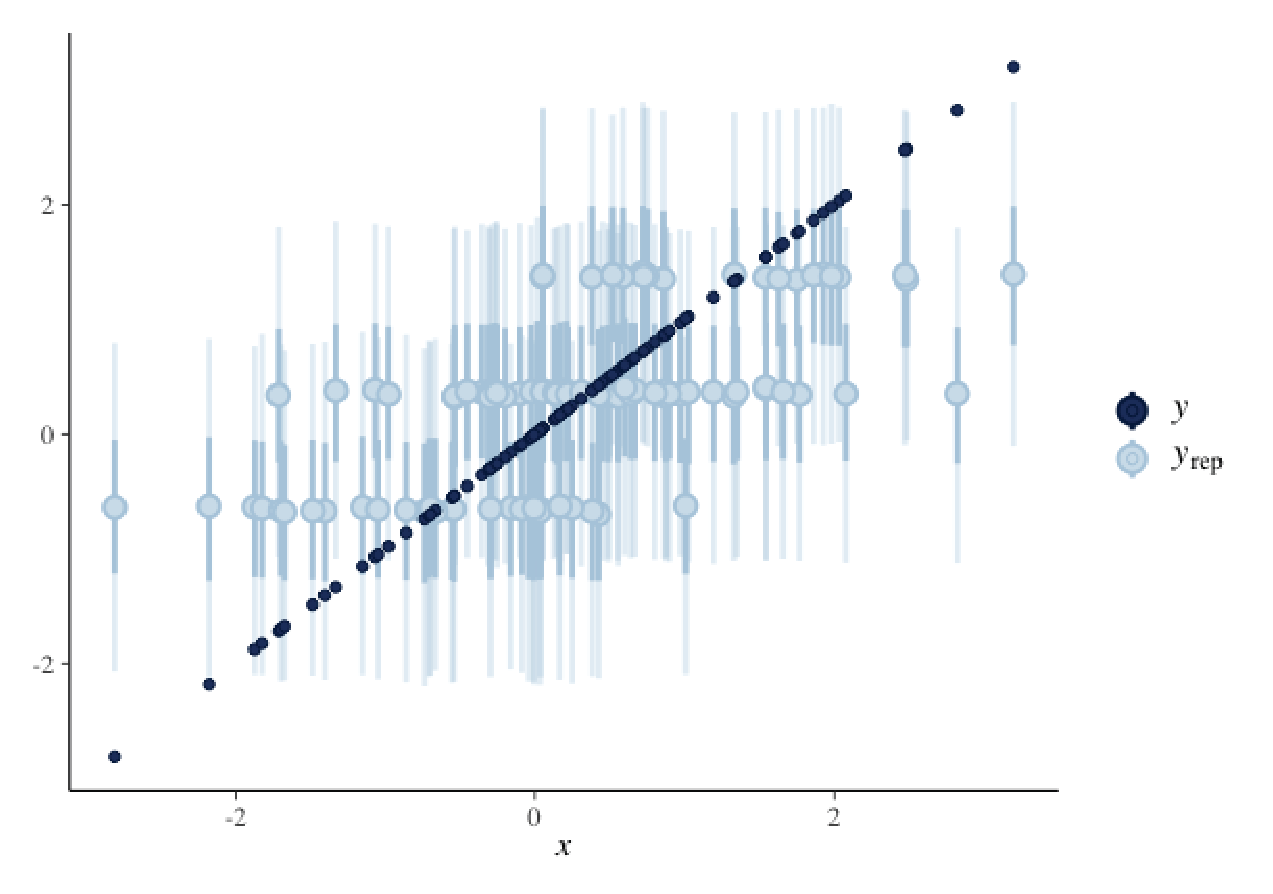
\includegraphics[height=6cm]{genomic-prediction-locus-1.eps}
  \end{center}
  \caption{Posterior prediction for locus 1. Small black dots indicate
    observed phenotypes. Large gray dots indicate the corresponding
    posterior prediction. The darker gray lines show the location of
    50\% credible intervals, and the lighter gray lines show the
    location of 90\% credible intervals.}\label{fig:locus-1}
\end{figure}

\begin{figure}
  \begin{center}
    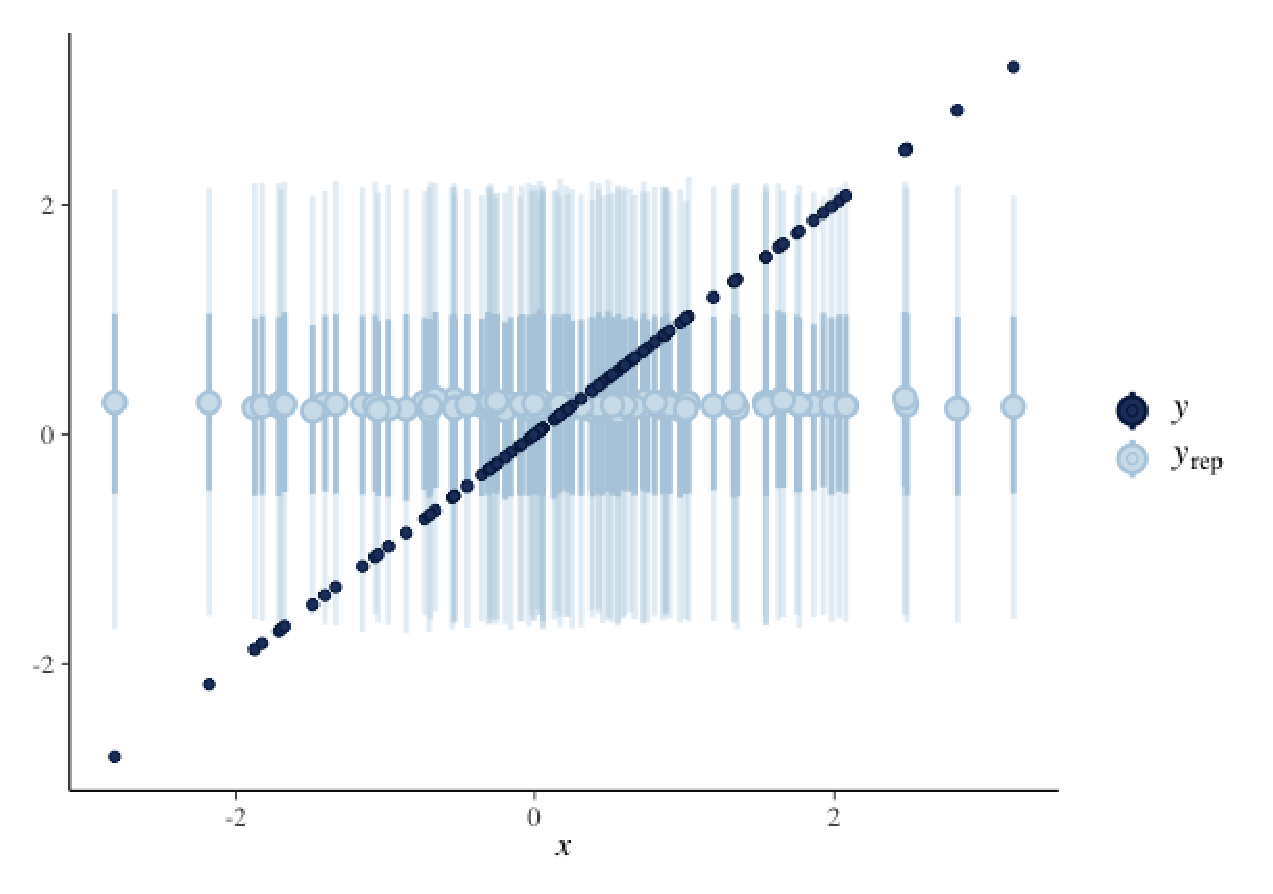
\includegraphics[height=6cm]{genomic-prediction-locus-17.eps}
  \end{center}
  \caption{Posterior prediction for locus 17.}\label{fig:locus-17}
\end{figure}

What about the multiple regression approach? First, take a look at the
estimated effects~(Table~\ref{table:multiple}). Not only does this
approach pick out the right loci, the first five, none of the other
loci have particularly large estimated effects. The largest, {\tt
  locus\_6} and {\tt locus\_8} are both only 0.07, as opposed to 0.14
in the locus by locus analysis. It would take much more extensive
simulation to demonstrate the advantage empirically, but it is clear
from first principles that multiple regression analyses will be more
reliable than locus by locus analyses because a multiple regression
analysis take account of random associations among loci.

Now compare phenotype predictions from the first five loci when each
effect is taken individually from Table~\ref{table:single} with the
prediction derived from the multple regression
approach~(Figure~\ref{fig:multiple}).\footnote{Use {\tt
    compare\_posterior\_predictions(fit\_list[1:5], fit)} to produce a
  similar plot using your results.} As you can see, using all 5 loci
together to predict phenotypes does a very good job of recovering
them. 

\begin{table}[ht]
\centering
\begin{tabular}{rrrr}
  \hline
 & mean & 2.5\% & 97.5\% \\ 
  \hline
locus\_2 & -0.96 & -1.07 & -0.86 \\ 
  locus\_1 & 0.92 & 0.84 & 1.00 \\ 
  locus\_3 & 0.48 & 0.39 & 0.56 \\ 
  locus\_4 & -0.44 & -0.52 & -0.36 \\ 
  locus\_5 & 0.23 & 0.15 & 0.32 \\ 
  locus\_6 & 0.07 & -0.03 & 0.16 \\ 
  locus\_8 & -0.07 & -0.15 & 0.02 \\ 
  locus\_11 & 0.06 & -0.03 & 0.15 \\ 
  locus\_14 & -0.06 & -0.14 & 0.03 \\ 
  locus\_20 & -0.06 & -0.14 & 0.03 \\ 
  locus\_12 & 0.05 & -0.04 & 0.14 \\ 
  locus\_7 & -0.04 & -0.12 & 0.04 \\ 
  locus\_18 & -0.03 & -0.10 & 0.06 \\ 
  locus\_16 & 0.02 & -0.07 & 0.10 \\ 
  locus\_10 & 0.02 & -0.07 & 0.11 \\ 
  locus\_19 & -0.02 & -0.10 & 0.06 \\ 
  locus\_17 & 0.01 & -0.08 & 0.09 \\ 
  locus\_9 & 0.01 & -0.08 & 0.09 \\ 
  locus\_15 & 0.00 & -0.07 & 0.08 \\ 
  locus\_13 & -0.00 & -0.09 & 0.09 \\ 
   \hline
\end{tabular}
\caption{Results from multiple regression analysis of simulated
  data.}\label{table:multiple} 
\end{table}

\begin{figure}
  \begin{center}
    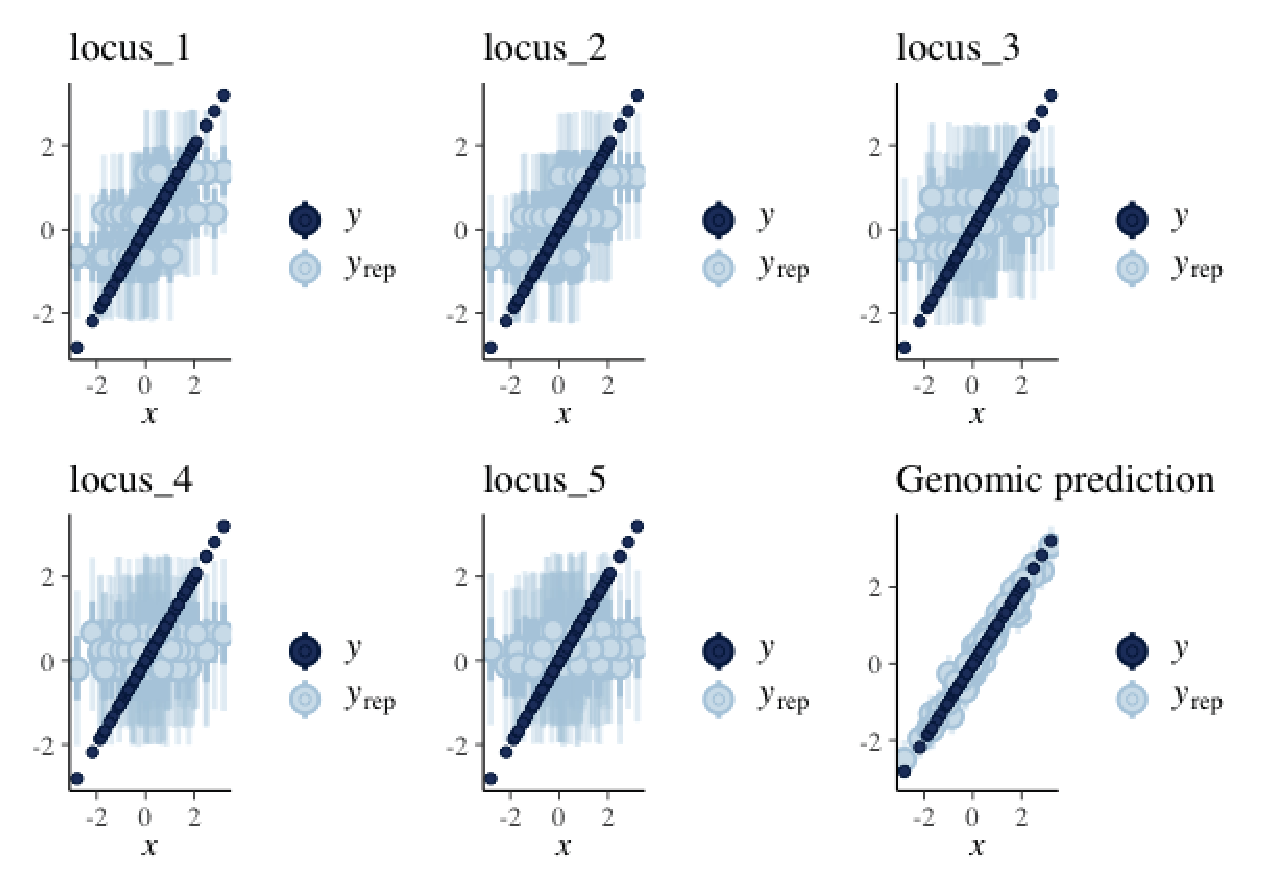
\includegraphics[height=6cm]{genomic-prediction-multiple.eps}
  \end{center}
  \caption{Posterior predictions for loci 1-5 from locus by locus
    regressions and the posterior preduction for the multiple
    regression.}\label{fig:multiple}
\end{figure}

\subsection*{CAUTION: Danger ahead!}\index{genomic prediction!caveats}

This all seems very promising, but a word of caution is in
order. Several papers, including one by Peter Turchin, have suggested
that there is strong evidence for selection on polygenic scores
associated with height using the same data set of 253,288 individuals
I referred to earlier~(references in Berg et
al.~\cite{Berg-etal-2018}). Specifically, these studies suggested (a)
that there is a cline in polygenic scores from south-to-north in
Europe (taller phenotypes predicted in the north) and (b) that the
cline is too steep to be accounted for by neutrual evolution. Berg et
al.~\cite{Berg-etal-2018} re-examined these claims using new data
available from the UK
Biobank~(\url{https://www.bdi.ox.ac.uk/research/uk-biobank}), which
includes a host of information on individual phenotypes as well as
genome-wide genotypes for the 500,000 individuals included in the
sample.\footnote{Although all of the samples are from the UK, one of
  the data sets Berg et al.~\cite{Berg-etal-2018} studied included
  individuals of European, but non-UK, ancestry.} They failed to
detect evidence of a cline in polygenic scores in their
analysis~(Figure~\ref{fig:UK-biobank}).

\begin{figure}
  \begin{center}
    \includegraphics[width=\textwidth]{UK-biobank.eps}
  \end{center}
  \caption{Polygenic score as a function of latitude and longitude for
    several different GWAS data sets.}\label{fig:UK-biobank}
\end{figure}

In thinking about this result, it's important to understand that Berg
et al.~\cite{Berg-etal-2018} did something a bit different from what
we did, but it's exactly what you'd want to do if polygenic scores
worked. They estiamted polygenic scores from each of the data sets
identified in the figure. Then they used those scores to estimate
polygenic scores for a new set of samples derived from the 1000
Genomes and Human Origins projects.\footnote{See Berg et
  al.~\cite{Berg-etal-2018} for details.} Think about it. A polygenic
score doesn't do us a whole lot of good if all it lets us do is to
predict (with uncertainty) a phenotype we already know. The hope is
that we can use the polygenic score to predict phenotypes for
individuals when we know their genotype but not their phenotype. What
this result shows is that extrapolation of a regression beyond the
range of variation included in the sample from which it was estimated
can be very problematic.

